\documentclass{beamer}
%
% Choose how your presentation looks.
%
% For more themes, color themes and font themes, see:
% http://deic.uab.es/~iblanes/beamer_gallery/index_by_theme.html
%
\mode<presentation>
{
  \usetheme{default}      % or try Darmstadt, Madrid, Warsaw, ...
  \usecolortheme{default} % or try albatross, beaver, crane, ...
  \usefonttheme{default}  % or try serif, structurebold, ...
  \setbeamertemplate{navigation symbols}{}
  \setbeamertemplate{caption}[numbered]
} 



\usepackage[english]{babel}
\usepackage[utf8]{inputenc}
\usepackage[T1]{fontenc}
\usepackage{graphicx}
\usepackage{fancyvrb}
\usepackage{listings}

\lstset{language=R,% set programming language
	basicstyle=\small,% basic font style
	keywordstyle=\bfseries,% keyword style
        commentstyle=\ttfamily\itshape,% comment style
	tabsize=3,% sizes of tabs
	showstringspaces=false,% do not replace spaces in strings by a certain character
	captionpos=b,% positioning of the caption below
        breaklines=true,% automatic line breaking
        escapeinside={(*}{*)},% escaping to LaTeX
        fancyvrb=true,% verbatim code is typset by listings
        extendedchars=false,% prohibit extended chars (chars of codes 128--255)
        literate={"}{{\texttt{"}}}1{<-}{{$\leftarrow$}}1{<<-}{{$\twoheadleftarrow$}}1
        {~}{{$\sim$}}1{<=}{{$\le$}}1{>=}{{$\ge$}}1{!=}{{$\neq$}}1{^}{{$^\wedge$}}1,% item to replace, text, length of chars
        alsoletter={.<-},% becomes a letter
        alsoother={$},% becomes other
        otherkeywords={!=, ~, $, *, \&, \%/\%, \%*\%, \%\%, <-, <<-, /},% other keywords
        deletekeywords={c}% remove keywords
}

%	numbers=left,% display line numbers on the left side
%	numberstyle=\scriptsize,% use small line numbers
%	numbersep=10pt,% space between line numbers and code

\usepackage{amsmath}
\DeclareMathOperator*{\argmax}{arg\,max}
\DeclareMathOperator*{\argmin}{arg\,min}

\title[]{Topic 2-1: Likelihood Construction $\&$ Estimation \\
Univariate Models}
\author{Department of Experimental Statistics \\
Louisiana State University}
\institute{}
\date{Date}

\setbeamertemplate{footline}[frame number]{}

\begin{document}

\begin{frame}[noframenumbering,plain]
  \titlepage
\end{frame}

% Uncomment these lines for an automatically generated outline.
%\begin{frame}{Outline}
%  \tableofcontents
%\end{frame}

\section{General Concept}

\begin{frame}{1. Introduction}
        \begin{itemize}
            \item Constructing the likelihood of the data is the foundation of model-based statistical inference.
            \item It leads to essentially automatic methods of inference, including point and interval estimation. 
            \item In this topic, we will focus on constructing the likelihood functions for various types of data, including discrete, continuous, mixture of discrete and continuous, and so on.
        \end{itemize}
    \end{frame}
%   \item A statistical model is a general functional relation between the unknown parameter(s) and the observed data.
%After a statistical model for the observed data has been formulated, the likelihood function of the data is the natural starting point for the inference in many statistical problems.
%\item The likelihood function typically leads to essentially automatic methods of inference, including point estimation, interval estimation, and hypothesis testing.
    \begin{frame}{Definition of Likelihood Functions}
        \begin{itemize}
            \item If random variables $\boldsymbol{Y} = (Y_{1}, \cdots, Y_{n})^{T}$ has {\it joint density (or joint probaility mass function)} $f(\boldsymbol{Y}; \boldsymbol{\theta})$ with unknown parameters $\boldsymbol{\theta} = (\theta_{1}, \cdots, \theta_{b})^{T}$, then the function of  $\boldsymbol{\theta}$ defined by 
$$
L(\boldsymbol{\theta}|\boldsymbol{Y}  = \boldsymbol{y}) = f(\boldsymbol{Y} = \boldsymbol{y};\boldsymbol{\theta}),
$$
where $\boldsymbol{y} = (y_{1}, \cdots, y_{n})^{T}$ is the observed data points from $\boldsymbol{Y}$, is the {\bf likelihood function}.
           \item  That is, the likelihood function is just the joint density (or probability mass function) evaluated at the observed data points.

        \end{itemize}
    \end{frame}


    \begin{frame}{Likeliihood Functions for IID Data}
        \begin{itemize}
            \item If the random variables $Y_{1}, \cdots, Y_{n}$ are indenpendent but each $Y_{i}$ can have a different density $f_{i}(Y_{i}; \boldsymbol{\theta})$, then the likelihood function becomes 
$$L(\boldsymbol{\theta}| \boldsymbol{y}) = \prod^{n}_{i=1}f_{i}(Y_{i} = y_{i};\boldsymbol{\theta}).$$
             \item If $Y_{1}, \cdots, Y_{n}$ are {\bf indenpendent and indentically distributed (iid)} random variables following density $f$, then the likelihood function becomes 
$$L(\boldsymbol{\theta}| \boldsymbol{y}) = \prod^{n}_{i=1}f(Y_{i} = y_{i};\boldsymbol{\theta}).$$
        \end{itemize}
    \end{frame}
    
        \begin{frame}{Discrete IID Random Variables: A Poisson Example}
        \begin{itemize}
            \item Fetal lamb movements data (Example 2.1): Leroux and Puterman (1992) give data on counts of movements in 240 five-second intervals of one fetal lamb:
            \begin{table}
\centering
\begin{tabular}{c|cccccccc}
No. of movements & 0 & 1 & 2 & 3 & 4 & 5 & 6 & 7 \\\hline
Widgets & 182 & 41 & 12 & 2 & 2 & 0 & 0 & 1 \\
\end{tabular}
\end{table}
    \item Suppose the counts of movements are from iid random variables $Y_{1}, \cdots, Y_{n}$  following the {\it Poisson probability mass function} with $\theta = \lambda$ and 
$$f(y;\lambda) = \frac{\lambda^{y}e^{-y}}{y!}, y = 0, 1, ....$$ 
Then, the likelihood function is 
$$L(\lambda|\boldsymbol{y}) = \prod^{n}_{i=1} f(y_{i};\lambda) = \prod^{n}_{i=1} \frac{\lambda^{{y}_{i}}e^{-\lambda}}{ y_{i}!} = \lambda^{n\bar{y}}e^{-n\lambda}\left( \prod^{n}_{i=1} y_{i}!   \right)^{-1},$$
where $\bar{y} = \sum^{n}_{i=1} y_{i}/n$.
        \end{itemize}
    \end{frame}
    
    



    \begin{frame}{Maximum Likelihood Estimator (MLE)}
        \begin{itemize}
            \item The value of $\boldsymbol{\theta}$ that maximizes the likelihood function $L(\boldsymbol{\theta}; \boldsymbol{y})$ is called the {\bf maximum likelihood estimator (MLE)} denoted by $\hat{\boldsymbol{\theta}}_{MLE}$, i.e.,
            
            $$\hat{\boldsymbol{\theta}}_{MLE} = \argmax_{\boldsymbol{\theta}} L(\boldsymbol{\theta}| \boldsymbol{y})$$
            
            .
            \item Such estimator is generally {\it optimal or at least optimal} in large samples (Fisher 1922), which we will discuss more in a future lecture.
            %\item In the following slides, we will focus on constructing likelihoods in a variety of situations.
        \end{itemize}
    \end{frame}
    
    \begin{frame}{Finding the MLE}
        \begin{itemize}
            \item In practice, $\hat{\boldsymbol{\theta}}_{MLE}$ is usually calculated by finding the optimizer of the {\bf log likelihood function} $\log(L(\boldsymbol{\theta}| \boldsymbol{y})).$
            
            \item If the likelihood function is differentiable in $\theta_{i}$ for $i = 1, \cdots, b,$  then the possible candidates for the MLE are the values of $(\theta_{1}, \cdots, \theta_{b})$ that solve 
             $$ \frac{\partial}{\partial \theta_{i}} \log(L(\boldsymbol{\theta}| \boldsymbol{y})) = 0\ \mbox{for}\ i = 1, \cdots, b.$$
             Solving the equations may give you {\it local or global minima, local or global maxima, or inflection points}. Then, some further arguments, such as checking that the second derivatives evaluated at the cadidate is less than 0, is needed for finding a global maximum.
        \end{itemize}
    \end{frame}
    
            \begin{frame}{The Poisson Example (Cont.)}
        \begin{itemize}
            \item Recall: The likelihood function from the Poisson example (page 5) is 
$L(\lambda|\boldsymbol{y}) = \lambda^{n\bar{y}}e^{-n\lambda}\left( \prod^{n}_{i=1} y_{i}!   \right)^{-1}.$
             \item The log likelihood function is $$\log\left[L(\lambda| \boldsymbol{y})\right] = n\bar{y}\log{\lambda} - n\lambda + \sum^{n}_{i=1}\log y_{i}!.$$
             \item Equate the derivative of the log likelihood with respect to $\lambda$ to zero, we obtain $\frac{n\bar{y}}{\lambda} - n = 0,$ i.e., the MLE candidate of $\lambda$ is $\bar{y} = \frac{86}{240} = .358$.
             \item Because the second derivative of the log likelihood function is $\frac{-n\bar{y}}{\lambda^{2}} < 0$ for all $\lambda,$ the function is {\it concave} and $\bar{y}$ is the global maximum. That is, $$\hat{\lambda}_{MLE} = \bar{y}.$$ 
        \end{itemize}
    \end{frame}


\begin{frame}[fragile]{Using R to find MLE: The Poisson Example}

\begin{lstlisting}
#data from the Poisson Example
count.v <- rep(c(0,1,2,3,4,5,6,7), c(182, 41, 12, 2, 2, 0, 0, 1)) 

#Log-likelihood function
poisson.log.like <- function(lambda,data){
  -sum(dpois(data, lambda, log = TRUE))
}

#Find MLE
fit.result <- nlminb(start = 0.5, objective = poisson.log.like, data = count.v, lower = 0, upper = Inf)
fit.result$par   
[1] 0.3583333

#theoretical MLE
mean(count.v) 
[1] 0.3583333
\end{lstlisting}
\end{frame}


\begin{frame}{A Multinomial Example}
        \begin{itemize}
            \item Consider $n$ independent trials, where each trail has $k \geq 2$ outcomes and has probability $p_{i}$ to be $i$-th outcome for $i = 1, \cdots, k$.
            \item Denote $N_{i}$ is the number of trials that are $i$-th outcome. Then, $(N_{1}, \cdots, N_{k})$ are distributed as a {\it multinomial distribution} with parameter $n$ and $ \textbf{p} = (p_{1}, \cdots, p_{k})$ with constraint $\sum^{k}_{i=1}p_{i} = 1$ denoted by $multinomial(n; \textbf{p} )$, and the likelihood of the observed trails $N_{1} = n_{1}, \cdots, N_{k} = n_{k}$ is 
            $$L(\textbf{p} | n_{1}, \cdots, n_{k}) = \frac{n!}{n_{1}!n_{2}!\cdots n_{k}!}p^{n_{1}}_{1} p^{n_{2}}_{2} \cdots p^{n_{k}}_{k}.$$
            \item  Binomial is a special case of the multinomial distribution with $k = 2.$
            \item See Example 2.2 for a k = 3 case. 
        \end{itemize}
    \end{frame}

    \begin{frame}[fragile]{Continuous IID Random Variables}
     Hurricane data: Larsen and Marx (2001) collect 36 hurricanes that had moved far inland on the East Coast of the U.S. in 1900-1969:

        
    \begin{lstlisting}
    > Hurr.rain 
    [1] 31.00 2.82 3.98 4.02 9.50 4.50 11.40 10.71 
    [9] 6.31 4.95 5.64 5.51 13.40 9.72 6.47 10.16 
    [17] 4.21 11.60 4.75 6.85 6.25 3.42 11.80 0.80
    [25] 3.69 3.10 22.22 7.43 5.00 4.58 4.46 8.00
    [33] 3.73 3.50 6.20 0.67
    \end{lstlisting}
    \begin{figure}
        \centering
        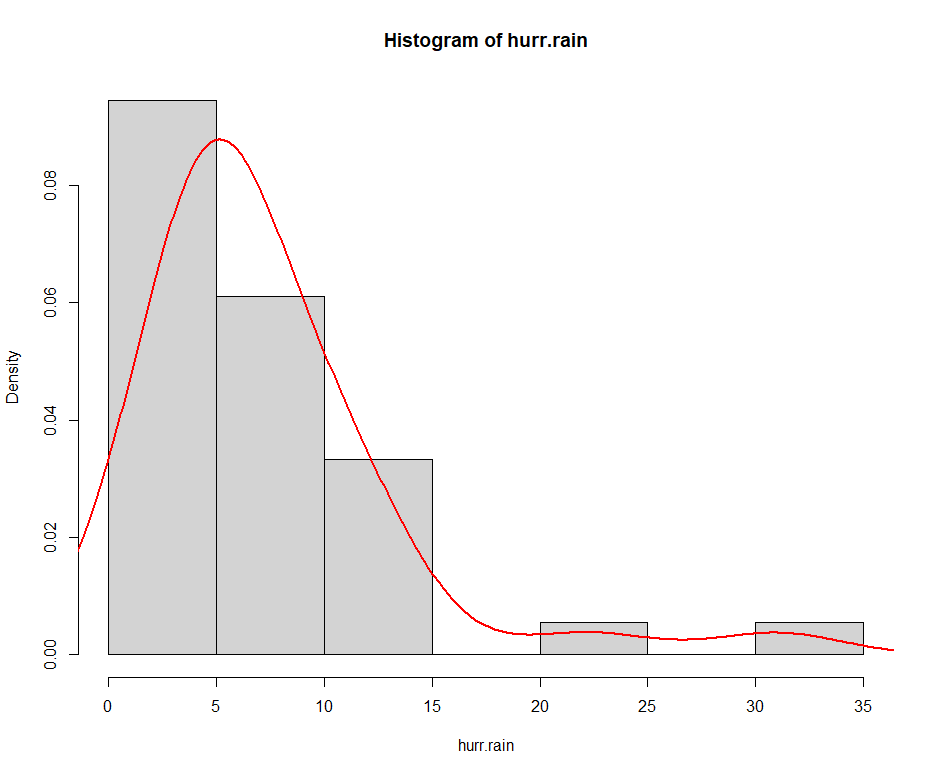
\includegraphics[width = 4 cm]{F1.png}
        \caption{Hurricane data}
        %\label{fig:my_label}
    \end{figure}
    \end{frame}
    
    \begin{frame}{Continuous IID Variables}
        \begin{itemize}
            \item  Consider iid sample data $y_{1}, \cdots, y_{n}$ from continuous random variable with density $f(y;\boldsymbol{\theta})$ 
            \item For example, if $f$ is the {\it gamma density} $f(y;\boldsymbol{\theta} = (\alpha, \beta)) = \frac{1}{\Gamma(\alpha)\beta^{\alpha}}y^{\alpha - 1}e^{-y/\beta},$ then the likelihood function is
            $$\prod^{n}_{i=1}\frac{1}{\Gamma(\alpha)\beta^{\alpha}}y^{\alpha - 1}_{i}e^{-y_{i}/\beta} = \{\Gamma(\alpha)\}^{-n}\beta^{-n\alpha}\{\prod^{n}_{i=1} y_{i}\}^{\alpha - 1} e^{-\sum^{n}_{i=1} y_{i}/\beta}$$ 
            and the log likelihood is 
            $$\ell(\boldsymbol{\theta}) = -n\log \Gamma(\alpha) - n\alpha\log \beta + (\alpha - 1) \sum^{n}_{i=1} \log y_{i} - \frac{\sum^{n}_{i=1} y_{i}}{\beta}.$$
        \end{itemize}
    \end{frame}
    
    \begin{frame}[fragile]{Using R to find MLE: The Hurricane Example}

\begin{lstlisting}
#data from the Hurricane Example
hurr.rain <- c(31.00, 2.82, 3.98, 4.02, 9.50, 4.50, 11.40, 10.71, 6.31, 4.95, 5.64, 5.51, 13.40, 9.72, 6.47, 10.16, 4.21, 11.60, 4.75, 6.85, 6.25, 3.42, 11.80, 0.80, 3.69, 3.10, 22.22, 7.43, 5.00, 4.58, 4.46, 8.00, 3.73, 3.50, 6.20, 0.67)
                
#Log-likelihood function
llik.gamma <- function(theta, dta=hurr.rain){
  -sum(dgamma(dta, shape=theta[1], scale=theta[2], log = TRUE))
}

#Find MLE
fit.result <- nlm(llik.gamma, c(1,2), dta=hurr.rain)
fit.result$estimate
[1] 2.187214 3.331863

\end{lstlisting}
\end{frame}

    
\begin{frame}{References}
        \begin{itemize}
                \item  More examples for constructing likelihood associated with iid data can be found in Section 7.2.2 of Casella and Berger (2002). 
                \begin{itemize}
                    \item Examples include Normal (7.2.5-6,7.2.11-12), Bernoulli (7.2.7), restricted MLE (7.2.8), Binomial (7.2.9) .
                    \item See how they argue the MLE is global maximum.
                \end{itemize}
               \item See Example 2.1 of the textbook for a {\it zero inflate Poisson distribution} example, and Example  2.2 for a multinomial example.
          \end{itemize}
    \end{frame}
    
    \begin{frame}{2. Connection of Discrete and Continuous Likelihood}
        \begin{itemize}
                \item  The continuous-data likelihood $\prod^{n}_{i=1}f(y_{i};\boldsymbol{\theta})$ looks the same as that for discrete data, but it is not a probability as it is for discrete data. (Note: It is from a density function, assigning zero probability to any single point)
                
                \item We can think the density evaluate at $Y = y$ as the limit probability on the small interval $[y - h, y + h],$ i.e.,
                $$f(y) = \lim_{h \rightarrow 0^{+}} \frac{F(y - h) - F(y - h)}{2h} = \lim_{h \rightarrow 0^{+}} \frac{P(Y \in (y - h, y + h))}{2h}$$
                \item If $Y$ now is a discrete random variable evaluated at $y$, then 
                $$\lim_{h \rightarrow 0^{+}} F(y+h) - F(y-h) = \lim_{h \rightarrow 0^{+}} F(y^{+}) - F(y^{-}) = f(y)$$
                \item More details can be found in section 2.2.3a of the textbook. This provides a unified perspective to connect discrete and continuous likelihood, and a broader definition of the likelihood is given in the next page. 
         \end{itemize}
    \end{frame}
    
    
     \begin{frame}{A Working Definition of the Likelihood}
        \begin{itemize}
            \item  Suppose $Y_{1}, \cdots, Y_{n}$ are independent random variables, and $Y_{i}$ has distribution function $F_{Y_{i}}(y_{i};\boldsymbol{\theta}).$
            \item The likelihood of data $\boldsymbol{y} = (y_{1}, \cdots, y_{n})$ observed from $(Y_{1}, \cdots, Y_{n})$ is
            \begin{equation}
            L(\boldsymbol{\theta}|\boldsymbol{y}) = \lim_{h \rightarrow 0^{+}} \left(\frac{1}{2h}\right)^{m}\prod^{n}_{i=1}\{F_{i}(y_{i}+h;\boldsymbol{\theta})-F_{i}(y_{i}-h;\boldsymbol{\theta})\}, \label{eq: working_def}
            \end{equation}
            where $1 \leq m \leq n$ depends on the number of continuous component in the data.
            \item In following slides, this general {\bf working definition of the likelihood function} is applied to more complicated examples.
        \end{itemize}
    \end{frame}
    

 

 \begin{frame}{3. Mixture of Discrete and Continuous components}
        \begin{itemize}
            \item  Some data $Y = y$, such as daily rainfall, often have a number of zeros (no rains), and the amounts greater than zero are best modeled by a continuous distribution.
            \item Such data are often modeled by
            a mixture of a point mass at zero $P(Y = 0) = 0$ and a continuous positive random variable $T$ having distribution function $F_{T}(y;\boldsymbol{\theta}).$ This means the distribution function of $Y$ is
            \begin{equation}
                F_{Y}(y;p, \boldsymbol{\theta}) = pI(0 \leq y) + (1-p)F_{T}(y;\boldsymbol{\theta}) \label{eq: mixture}
            \end{equation}
            
        \end{itemize}
    \end{frame}
    

    
    
    
 \begin{frame}{Mixture of Discrete and Continuous components (Cont.)}
        \begin{itemize}
            \item Suppose there are iid data $y_{1}, \cdots, y_{n}$ from the mixture density (\ref{eq: mixture}), and $n_{0}$ observations of the data are 0.
            \item By the working definition of the likelihood  (\ref{eq: working_def}), the likelihood function of $y_{1}, \cdots, y_{n}$ is
       \begin{small}
        \begin{eqnarray}
       L(\boldsymbol{\theta}|\boldsymbol{y})  & = & \lim_{h \rightarrow 0^{+}} \left(\frac{1}{2h}\right)^{m}\prod^{n}_{i=1}\{F_{Y}(y_{i}+h; p, \boldsymbol{\theta}) - F_{Y}(y_{i}-h; p, \boldsymbol{\theta})\}\nonumber\\
        & = & \lim_{h \rightarrow 0^{+}} \{F_{Y}(h; p, \boldsymbol{\theta}) - F_{Y}(h; p, \boldsymbol{\theta})\}^{n_{0}} \times \nonumber\\ 
        & & \lim_{h \rightarrow 0^{+}} \prod^{n}_{Y_{i} > 0}\left\{\frac{F_{Y}(y_{i}+h; p, \boldsymbol{\theta}) - F_{Y}(y_{i}-h; p, \boldsymbol{\theta})}{2h}\right\}\nonumber\\
        & = & \lim_{h \rightarrow 0^{+}} \{p + (1-p)F_{T}(h; \boldsymbol{\theta})\}^{n_{0}} \times \nonumber\\
       & &  \prod^{n}_{Y_{i} > 0}\left\{\frac{(1-p)F_{T}(y_{i}+h; \boldsymbol{\theta}) - (1-p)F_{T}(y_{i}-h; \boldsymbol{\theta})}{2h}\right\} \nonumber\\ 
       & = & p^{n_{0}}(1-p)^{n-n_{0}} \prod^{n}_{y_{i} > 0} f_{T}(y_{i}:\boldsymbol{\theta}) \nonumber
            \end{eqnarray}
        \end{small}
        \end{itemize}
    \end{frame}

 \begin{frame}{4. Proportional Likelihoods}
        \begin{itemize}
        \item Suppose there are data $y_{1}, \cdots, y_{n}$ from a continuous distribution with density $f_{Y}(y;\boldsymbol{\theta})$. 
        \item We are interested in constructing the likelihood of the transformed data $x_{i} = g(y_{i})$ for $i = 1, \cdots, n,$ where $g$ is a known, increasing, continuously differentiable function. 
        \item Note: The assumptions of $g$ implies $g$ is one-to-one function and its inverse function $g^{-1}$ exists.
        \item The likelihood inference based on one dataset $(x_{1}, \cdots, x_{n})$ should be identical to inference based on dataset $(y_{1}, \cdots, y_{n})$. (why?)
        \end{itemize}
    \end{frame}
    
\begin{frame}{Proportional Likelihoods (Cont.)}
        \begin{itemize}
        \item Denote $g^{-1} = h,$ the likelihood of $(x_{1}, \cdots, x_{n})$
            \begin{eqnarray}
        L(\boldsymbol{\theta}|\boldsymbol{x})  & = & \prod^{n}_{i=1}f_{Y}(h(x_{i};\boldsymbol{\theta}))h'(x_{i})   \nonumber\\
        & = & \prod^{n}_{i=1}f_{Y}(h(x_{i};\boldsymbol{\theta}))h'(g(y_{i}))\nonumber\\
        & = & \prod^{n}_{i=1}f_{Y}(h(x_{i};\boldsymbol{\theta}))\frac{1}{g'(y_{i})} \\\nonumber
        & & (since \frac{dh(x)}{dx} = \frac{dg^{-1}(x)}{dx} = \frac{1}{g'(g^{-1}(x))})\nonumber\\
        & = & L(\boldsymbol{\theta}|\boldsymbol{y}) \frac{1}{g'(y_{i})}.\nonumber
            \end{eqnarray}
            \item The two likelihoods are proportional as functions of $\boldsymbol{\theta}$ for all $y_{i}$, \item This implies that maximum likelihood estimates and likelihood ratio tests are identical whether derived from        $L(\boldsymbol{\theta}|\boldsymbol{x})$ or        $L(\boldsymbol{\theta}|\boldsymbol{y})$. 
        \end{itemize}
    \end{frame}

 \begin{frame}{5. The Empirical Distribution Function as an MLE}
        \begin{itemize}
            \item In some situation, we do not know how to model the data with a parametric distribution. 
            \item We only know data $y_{1}, \cdots, y_{n}$ are iid from a continuous but unknown distribution whose distribution function is $F(y)$, i.e., the parameter space is the set of all distribution functions.
            \item Ignoring the factor $(2h)^{-m}$ in the working definition of the likelihood, an approximate likelihood for $F$ is
            $$L_{h}(F|\boldsymbol{y}) = \prod^{n}_{i=1}\{F(y_{i} + h) - F(y_{i} - h)\},$$
            where $h$ is assumed to be a small positive constant.
        \end{itemize}
    \end{frame}

    \begin{frame}{The Empirical Distribution Function as an MLE (Cont.)}
        \begin{itemize}
            \item Assume there are no ties in the sample and $h$ is small enough to ensure that $[Y_{i} + h, Y_{i} + h]$ does not contain $Y_{j}$ for any $j \neq i$.
            \item Denote $p_{i, h} = F(y_{i} + h) - F(y_{i} - h)$. Then, $L_{h}(F|\boldsymbol{y})$ becomes $\prod^{n}_{i=1} p_{i, h}$.
            \item Since increasing $p_{i,h}$ increases $L_{h}(F|\boldsymbol{y}),$ we want $p_{i,h}$ to be as large as possible while still satisfying $\sum^{n}_{i=1} p_{i,h} \leq 1.$ This implies $p_{i,h} > 0$ and $\sum^{n}_{i=1} p_{i,h} = 1.$
        \end{itemize}
    \end{frame}


    \begin{frame}{The Empirical Distribution Function as an MLE (Cont.)}
        \begin{itemize}
            \item To maximize the likelihood subject to $p_{i,h} > 0$ and $\sum^{n}_{i=1} p_{i,h} = 1,$ we can use the method of Lagrage multipliers to find the stationary points of 
            $$g(p_{1,h}, \cdots, p_{n,h}, \lambda) = \sum^{n}_{i=1}\log(p_{i,h}) + \lambda (\sum^{n}_{i=1}p_{i,h}-1).$$
            \item The stationary points satisfies
            \begin{eqnarray}
                \frac{\partial g}{\partial p_{i,h}}    & = & \frac{1}{p_{i,h}} + \lambda = 0, i = 1, \cdots, n. \nonumber \\
                \frac{\partial g}{\partial \lambda} & = & \sum^{n}_{i=1} p_{i,h} - 1 = 0. \nonumber
            \end{eqnarray}
        \end{itemize}
    \end{frame}
    
        \begin{frame}{The Empirical Distribution Function as an MLE (Cont.)}
        \begin{itemize}
            \item The first $n$ equations implies $ p_{i,h} = -1/\lambda,$ which upon substitution into the last equation yields $\lambda = -n$. Thus, the MLE of $p_{i,h} = F(y_{i} + h) - F(y_{i} - h)$ satisfies
            $$\hat{F}_{h}(y_{i} + h) - \hat{F}_{h}(y_{i} - h) = \frac{1}{n}.$$
            This means the MLE puts the equal probability mass $1/n$ on the $n$ observed values.
            \item By Problem 2.10 of the textbook, 
            $\hat{F}_{h}(y) \rightarrow \frac{1}{n} \sum^{n}_{i=1}I(Y_{i} \leq y),$ which is called the empirical distribution function.
            \item Thus, we take 
            $$\hat{F}_{MLE}(y) = \frac{1}{n} \sum^{n}_{i=1}I(y_{i} \leq y).$$
            as the MLE of $F(y)$.
        \end{itemize}
    \end{frame}

    \begin{frame}{6. Likelihood for Type I Censoring}
        \begin{itemize}
            \item Lawless (1982) gives data on pieces of equipment that are started at different times and later regularly checked for failure. 
            \item When the study is ended, there are three of the items had not failed. For the three items, we can only know their failure time is greater than the ended time of the study but not exact failure time. Such data is called \textbf{right censored data}. 
            \item The data in days is recorded below
      
            \begin{small}
            \begin{table}
            \begin{tabular}{|p{3 cm}|c|c|c|c|c|c|c|c|c|c|}
                \hline
                Observed time & 2 & 72 & 51 & 60 & 33 & 27 & 14 & 24 & 4 & 21 \nonumber\\
                \hline
                Failure (1) or Right Censored (0) & 1 & 0 & 1 & 0 & 1 & 1 & 1 & 1 & 1 & 0 \nonumber\\
                 \hline
            \end{tabular}
            \end{table}
            \end{small}
        \end{itemize}
    \end{frame}

    

   \begin{frame}{Likelihood for Type I Censoring (Cont.)}
        \begin{itemize}
            \item Given a random variable $X$, we might observe it if $X \leq R_{0}$ (Right censoring) or $X \geq L_{0}$ (Left censoring), i.e. we observe all values of $X$ in some specified time period. Such type of censoring is called {\bf Type I Censoring}.
            \item Suppose $X$ has density $f(x;\boldsymbol{\theta})$ with distribution function $F(x;\boldsymbol{\theta}),$ and that $y_{i}$ is independently observed data from 
            $$Y = \left\{\begin{array}{cc}
                 L_{0}, X_{i} \leq L_{i},  \\
                 X_{i}, L_{0} <  X_{i} < R_{0},  \\
                 R_{0}, X_{i} \geq R_{0}.  \\
            \end{array}\right.$$
            for $i = 1, \cdots, n.$
            \item The likelihood function of $y_{1}, y_{2}, \cdots, y_{n}$ is 
            $$\{F(L_{0};\boldsymbol{\theta})\}^{n_{L}}\{\prod_{L_{0} < y_{i} < R_{0}} f(y_{i};\boldsymbol{\theta})\}\{1-F(R_{0}; \boldsymbol{\theta})\}^{n_{R}}$$
            if there are $n_{L}$ left censoring data and $n_{R}$ right censoring data.
        \end{itemize}
    \end{frame}
    
    
    \begin{frame}{Likelihood for Random Censoring}
        \begin{itemize}
            \item In previous situation, the censoring times $L_{0}$ and $R_{0}$ were considered fixed. In medical studies, however, patients often enter the studies at different times that are modeled as random variables.
            \item For illustration, we only consider the random right censoring times $R_{1}, \cdots, R_{n}$. 
            \item Define the random observing time  $Y_{i} = min(X_{i}, R_{i})$ and $\Delta_{i} = I(X_{i} \leq R_{i}),$ and assume the censoring times are independent of $X_{1}, \cdots, X_{n}$ and are iid with distribution $G(t)$ and density $g(t)$.
        \end{itemize}
    \end{frame}
    
    
        \begin{frame}{Likelihood for Random Censoring}
        \begin{itemize}
            \item The likelihood due to $(Y_{i} = y_{i}, \delta = 1)$ is $\frac{P(Y_{i} \in (y_{i} - h, y_{i} + h], \delta_{i} = 1)}{2h}$
            \begin{eqnarray}
             & = &      \frac{P(Y_{i} \in (y_{i} - h, y_{i} + h], X_{i} \leq R_{i})}{2h} \nonumber \\
            & = &     \frac{1}{2h} \int^{\infty}_{-\infty}\int^{\infty}_{-\infty}\left[I(y-h < t \leq y + h, t \leq r)f(t,\boldsymbol{\theta})g(r)\right]dtdr \nonumber\\
         & = &     \frac{1}{2h} \int^{y_{i}+h}_{-y_{i}-h}\left[\int^{\infty}_{-\infty}I( t \leq r)g(r)dr\right]f(t,\boldsymbol{\theta})dt \nonumber\\
         & = &     \frac{1}{2h} \int^{y_{i}+h}_{y_{i}-h}\left(1-G(t)\right)f(t,\boldsymbol{\theta})dt \nonumber\\
         & \rightarrow &
         [1-G(y_{i})]f(y_{i};\boldsymbol{\theta}) \nonumber
            \end{eqnarray}
as $h \rightarrow 0$. Note the last line is by the Fundamental Theorem of Calculus.
        \end{itemize}
    \end{frame}
    
    
            \begin{frame}{Likelihood for Random Censoring}
        \begin{itemize}
            \item A analogous argument can be used to argue the likelihood contributed from data $(Y_{i} = y_{i}, \delta = 0)$ is 
            $$\frac{P(Y_{i} \in (y_{i} - h, y_{i} + h], \delta_{i} = 1)}{2h} \rightarrow [1-F(y; \boldsymbol{\theta})] g(y).$$
            (See pages 49-50 of the textbook and checked by yourself.)
            
            \item Put the two types of likelihood together, the likelihood for the iid data $\boldsymbol{y} = (y_{1}, \cdots, y_{n})$ and $\boldsymbol{\delta} = (\delta_{1}, \cdots, \delta_{n})$ is  
   \begin{small}
     \begin{eqnarray}
         L(\boldsymbol{\delta}| \boldsymbol{y}, \boldsymbol{\delta})    & = &   \left\{\prod^{n}_{i=1}f(y_{i};\boldsymbol{\delta})^{\delta_{i}}\left[1-F(y_{i};\boldsymbol{\delta})\right]^{1-\delta_{i}}\right\} \nonumber\\
        & & \times \prod^{n}_{i=1}\{g(y_{i})^{1-\delta_{i}}[1-G(Y_{i})]^{\delta_{i}}\} \nonumber\\
        & = &  \prod^{n}_{i=1}\left\{f(y_{i};\boldsymbol{\delta})^{\delta_{i}}\left[1-F(y_{i};\boldsymbol{\delta})\right]^{1-\delta_{i}}g(y_{i})^{1-\delta_{i}}[1-G(Y_{i})]^{\delta_{i}}\right\}  \nonumber
            \end{eqnarray}
   \end{small}
      \item Note that the unknown censoring distribution $G$ is not needed to estimate $\boldsymbol{\theta}$.

            
        \end{itemize}
    \end{frame}
    
    \begin{frame}{Revisit Lawless (1982) data}
        \begin{itemize}
            \item There are $n = 10$ data points with $n_{R} = 3$ right censoring data.
            \begin{small}
            \begin{table}
            \begin{tabular}{|p{3 cm}|c|c|c|c|c|c|c|c|c|c|}
                \hline
                $\boldsymbol{y}:$ Observed time & 2 & 72 & 51 & 60 & 33 & 27 & 14 & 24 & 4 & 21 \nonumber\\
                \hline
                $\boldsymbol{\delta}:$ Failure (1) or Right Censored (0) & 1 & 0 & 1 & 0 & 1 & 1 & 1 & 1 & 1 & 0 \nonumber\\
                 \hline
            \end{tabular}
            \end{table}
            \end{small}
            \item Find MLE
            \begin{eqnarray}
            L(\sigma|\boldsymbol{y}, \boldsymbol{\delta}) & = & \prod^{n}_{i=1}\left[\frac{1}{\sigma}\exp(-Y_{i}/\sigma)\right]^{\delta_{i}} \left[\exp(-y_{i}/\sigma)\right]^{1-\delta_{i}} \nonumber\\
            & = & \left(\frac{1}{\sigma}\right)^{n-n_{R}}\exp(-n\bar{y}/\sigma) \nonumber\\
        \ell (\sigma)    & = & \log(L(\sigma|\boldsymbol{y})) = -(n-n_{R})\log \sigma - \frac{n\bar{y}}{\sigma} \nonumber\\
        \hat{\sigma}_{MLE} & = & \left(\frac{n}{n-n_{R}}\right)\bar{y} = 44.0 \nonumber
            \end{eqnarray}
        \end{itemize}
    \end{frame}


    \begin{frame}{ Main Reference and Homework}
        \begin{itemize}
            \item HW1 has been posted on ... and the due day is ...
        \end{itemize}
    \end{frame}


\end{document}


    
\begin{frame}{Introduction}

\begin{itemize}
  \item Your introduction goes here!
  \item Use \texttt{itemize} to organize your main points.
\end{itemize}

\vskip 1cm

\begin{block}{Examples}
Some examples of commonly used commands and features are included, to help you get started.
\end{block}

\end{frame}

\section{Some \LaTeX{} Examples}

\subsection{Tables and Figures}

\begin{frame}{Tables and Figures}

\begin{itemize}
\item Use \texttt{tabular} for basic tables --- see Table~\ref{tab:widgets}, for example.
\item You can upload a figure (JPEG, PNG or PDF) using the files menu. 
\item To include it in your document, use the \texttt{includegraphics} command (see the comment below in the source code).
\end{itemize}

% Commands to include a figure:
%\begin{figure}
%\includegraphics[width=\textwidth]{your-figure's-file-name}
%\caption{\label{fig:your-figure}Caption goes here.}
%\end{figure}

\begin{table}
\centering
\begin{tabular}{l|r}
Item & Quantity \\\hline
Widgets & 42 \\
Gadgets & 13
\end{tabular}
\caption{\label{tab:widgets}An example table.}
\end{table}

\end{frame}

\subsection{Mathematics}

\begin{frame}{Readable Mathematics}

Let $X_1, X_2, \ldots, X_n$ be a sequence of independent and identically distributed random variables with $\text{E}[X_i] = \mu$ and $\text{Var}[X_i] = \sigma^2 < \infty$, and let
\[ S_n = \frac{X_1 + X_2 + \cdots + X_n}{n}
      = \frac{1}{n}\sum_{i}^{n} X_i \]
denote their mean. Then as $n$ approaches infinity, the random variables $\sqrt{n}(S_n - \mu)$ converge in distribution to a normal $\mathcal{N}(0, \sigma^2)$.

\end{frame}



\begin{frame}[fragile]{An R Example}
\begin{large}
    Contexte : \newline
\end{large}

\begin{itemize}
    \item Avertir Drupal
\end{itemize}
\begin{lstlisting}

count.v <- rep(c(0,1,2,3,4,5,6,7), c(182, 41, 12, 2, 2, 0, 0, 1)) #data

poisson.log.like<-function(lambda,data){
  -sum(dpois(data, lambda, log = TRUE))
}

fit.result <- nlminb(start = 0.5, objective = poisson.log.like, data = count.v,
                     lower = 0, upper = Inf)
fit.result$par #MLE    
  
mean(count.v) #theoretical MLE
\end{lstlisting}
\end{frame}


   \begin{frame}{Numerical Examples}
        \begin{itemize}
            \item Leroux and Puterman (1992, p. 546)
give data on counts of movements in five-second intervals of one fetal lamb (n = 240 intervals):
\begin{table}
\centering
\begin{tabular}{c|cccccccc}
No. of movements & 0 & 1 & 2 & 3 & 4 & 5 & 6 & 7 \\\hline
Widgets & 182 & 41 & 12 & 2 & 2 & 0 & 0 & 1 \\
\end{tabular}
\item Suppose all interval counts are independent Poisson random variables with parameter $\lambda$. Then the MLE of $\lambda$ is $\bar{y} = \frac{86}{240}$ 
\end{table}
%\caption{\label{tab:widgets}An example table.}
           \item 
        \end{itemize}
    \end{frame}


  
    \begin{frame}{Finding MLEs from the differentiable likelihood functions}
        \begin{itemize}
            \item Denote the log likelihood function $\log(L(\boldsymbol{\theta}; \boldsymbol{y}))$ by $\ell(\boldsymbol{\theta})$, and assume $\ell(\boldsymbol{\theta})$ is differentiable with respect to $\boldsymbol{\theta}$. 
            \item The procedure for obtaining the MLE from $\ell(\boldsymbol{\theta})$ is
\begin{enumerate}
\item Differentiate  $\ell(\boldsymbol{\theta})$ with respect to $\boldsymbol{\theta}$ to obtain the likelihood score function $S(\boldsymbol{\theta}) = (\frac{\partial \ell(\boldsymbol{\theta})}{\partial \theta_{1}}, \cdots, \frac{\partial \ell(\boldsymbol{\theta})}{\partial \theta_{b}})^{T}$.
\item Find possible MLE cadidates by solving the likelihood equations $S(\boldsymbol{\theta}) = \boldsymbol{0}_{b \times 1}.$
\item Check if the solution from the last step is the global maximizer of  $\ell(\boldsymbol{\theta})$. If it is, then the solution is the MLE of $\ell(\boldsymbol{\theta})$.
\end{enumerate}
        \end{itemize}
    \end{frame}
